\textit{
Things implicitly assumed in the following that I will write in previous sections:
\begin{enumerate}
    \item The dust cycle
    \item A conclusion on what the full H-ATLAS survey provides
\end{enumerate}
}

\section{Introduction}

\section{Interstellar Dust as a Tracer of Cosmic Evolution}

Interstellar dust is responsible for obscuring approximately half of all starlight since the Big Bang (\citealt{Puget_1996}; \citealt{Fixsen_1998}; \citealt{Dole_2006}; \citealt{Driver_2016}). Assuming that young, massive stars are the main culprit for the heating of the interstellar dust and produce the UV photons that get absorbed and reradiated to far-IR wavelengths (\citealt{Kennicutt_1998}; \citealt{Calzetti_2007}; \citealt{Kennicutt_2009}), then measuring extragalactic dust masses is useful in our understanding of obscured star formation at different times in cosmic history. This naturally results from dust being a by-product of star formation. In order to study the evolution in the star formation rate density of the Universe, the most direct method is to measure the mass of galaxies' molecular gas reservoirs from which the stars form and estimate the star formation activity from the evolution of the cosmic molecular gas mass density. As detailed in the subsequent Chapter, molecular hydrogen, $H_2$ (the main component of the molecular gas), cannot be easily observed from the cold ISM ({\color{red} Typical temperature range}), whereas dust emission provides a suitable alternative at these temperatures. Using independent measures of the cosmic gas mass density from dust-traced gas mass (assuming some gas-to-dust mass ratio) allows us to constrain both the contribution of obscured star formation and the dust content of galaxies over time. In addition, metals are produced and expelled during supernovae and from stellar winds, with some fraction becoming bound to dust grains in the ISM. Here they may be ejected from the galaxy by starburst winds or become part of the next generation of stars. As a result, the total dust mass is a fundamental property of the ISM that can be used to trace the evolutionary stage of the galaxy, especially when used in conjunction with stellar and gas masses (e.g. \citealt{Cortese_2012}; \citealt{deVis_2017a}; \citealt{deVis_2017b}).

For these reasons, studying the distribution of dust masses for a population of galaxies across time can provide important insights into the properties and evolution of galaxies and their ISM. The dust mass function (DMF), the space density of galaxies as a function of dust mass, is a fundamental measure of the dust content of galaxies, providing crucial information on galaxy evolution, star formation activity and the cosmic dust budget. In this study we use the results of the crossmatching analysis of the South Galactic Pole field of the \textit{Herschel}-ATLAS survey, as presented in the previous Chapter, to derive the far-IR selected DMF and investigate whether it has evolved with redshift from the local DMF to z $\sim$ 1.

\section{Local and High Redshift DMFs in the Literature}

Using surveys selected from sub-mm wavelengths provides a number of advantages when determining the DMF. At longer sub-mm wavelengths we sample the Rayleigh-Jeans tail of the Planck function where the flux density is least sensitive to the temperature of the dust and most sensitive to the dust's mass. Prior to the surveys conducted with \textit{Herschel}, \textit{Planck} and SCUBA in the local Universe, estimates of the local DMF often started from local \textit{IRAS} 60\,\micron luminosity functions (LF) and extrapolating this to sub-mm wavelengths on the assumption of an average FIR SED with a single dust temperature and dust emissivity index $\beta$ for all galaxies (see Chapter \ref{chapter:Dust_Evolution} for detail on the role of dust temperature and $\beta$ on the FIR SED). Naturally this lead to high dependence on the assumed dust temperature and $\beta$ value. Given that temperature evolves with luminosity (see our study on the temperature evolution with redshift for dusty star forming galaxies, DSFGs; Figure \ref{fig:wavepeak_lir}), extrapolating from one wavelength to another inherently contained a bias at high and low luminosity scales, causing a distortion in any DMF measured from the translation of such a luminosity function (\citealt{Dunne_2000}). The advent of \textit{Herschel} and \textit{Planck} allowed for large samples detected at far-IR wavelengths closer to the peak of the dust emission, enabling estimates of the DMF directly from sub-mm wavebands. The disadvantage of these long wavelength derived DMFs is the large beam size at these operating wavebands, causing blending and source misidentification (as illustrated through the use of the Likelihood Ratio method in the previous chapter).

The first direct measurements of the sub-mm derived DMF were with SCUBA using the SCUBA Local Universe Galaxy Survey (SLUGS: \citealt{Dunne_2000}; \citealt{Dunne_2001}; \citealt{Vlahakis_2005}), a survey of local \textit{IRAS}-selected galaxies. However, these studies were limited by small number statistics and were limited to very small redshifts. A high redshift (z = 2.5) DMF for comparison with the local SLUGS DMF was presented in \citealt{Dunne_2003}, suggesting that galaxies with the highest dust masses have an order of magnitude more dust than locally (assuming pure dust mass evolution and no evolution in the number density of the most massive galaxies). An obvious drawback of these studies is that even when extapolations of the \textit{IRAS} 60\,\micron LF are no longer required, the SLUGS studies depended on sub-mm observations of samples of galaxies selected in other wavebands. Improvements were made with the introduction of the Balloon-borne Large Aperture Submillimeter Telescope (BLAST; \citealt{Devlin_2009}), which allowed for the detection and derivation of the DMF from a sample of galaxies selected from wavelengths spanning the peak of the FIR background (the operating wavelengths of BLAST were 250, 350 and 500\,\micron, as it was designed as a precursor to the \textit{Herschel}-SPIRE instrument). \citealt{Eales_2009} used BLAST data to arrive at similar conclusions, that there is strong evolution in the LF in the three BLAST bands and in the DMF out to z = 1. The concurrence of the two suggesting that the evolution in the sub-mm luminosity of these galaxies is directly related to the increase in their dust reservoirs. However, this study was also limited by small number statistics ($\sim$ 100 sources).

The first study to measure the evolution in the DMF using the large H-ATLAS survey was \citealt{Dunne_2011}, using a 250\,\micron selected sample of 1867 sources from the SDP. This represented an order of magnitude larger than previous studies, allowing for a significant direct measurement of the density of galaxies as a function of dust mass to a redshift of 0.5. The main conclusions about the DMF between 0 < z < 0.5 from this study were that dust masses of the most massive galaxies decreased by a factor of 4 or 5 over the past 5 billion years and the integrated dust density evolves with redshift according to $\rho_{\textrm{dust}} \propto (1+z)^{4.5}$. The local density is estimated to be $\rho_{\textrm{dust}, (z=0)} = 9.8\times10^4$\,$M_\odot$ Mpc$^{-3}$. This work was developed further in \citealt{Beeston_2018} by deriving the local (z < 0.1) DMF for the largest sample of galaxies at the time of writing ($\sim$ 16,000 galaxies), utilizing the crossmatching between the H-ATLAS and the GAMA spectroscopic survey detailed in \citealt{Bourne_2016}. The sample size of \citealt{Beeston_2018} permitted dust masses as low as $\sim$ $10^4$\,$M_\odot$ and therefore extended the observed range of the DMF by at least an order of magnitude at the lowest masses compared to previous measurements. This yielded better constraints on the low mass end of the DMF which despite accounting for a negligible amount of the dust budget compared to the most massive galaxies, contribute substantially in number. There are a wide range of predictions for the slope of the low dust mass end of the DMF as this regime is constrained by sources that tend to be nearby and faint, and suffer from low numbers in flux-limited surveys such as H-ATLAS. With the size of the \citealt{Beeston_2018} sample the measurements of the low mass end of the DMF in this study are currently our best estimate. Despite differences in the measured low mass slope of \citealt{Dunne_2011} and \citealt{Beeston_2018}, both have local dust mass densities (DMD) in good agreement.

More recently, \citealt{Driver_2018} produced an extended DMF and measure of the DMD out to z = 5. This study was based on an optically-selected sample of approximately 570,000 galaxies from GAMA, G10-COSMOS (\citealt{Davies_2015}; \citealt{Andrews_2017}) and 3D-HST (\citealt{Brammer_2012}; \citealt{Momcheva_2016}). While \citealt{Dunne_2011} had observed a decline in the DMD in the highest redshift bin of their study (z = 0.4 -- 0.5), this was postulated to be the result of incompleteness. The wealth of data in \citealt{Driver_2018} enabled the peak in the DMD to be constrained closer to z $\sim$ 1, corresponding to a lookback time of approximately 8\,Gyr. This could mean that the DMD coincides (or trails behind by the order of 1 -- 2 Gyr) with the peak epoch of star formation which is known to peak at z $\sim$ 2 (\citealt{Cucciati_2012}; \citealt{Burgarella_2013}; \citealt{Madau_2014}). Unlike \citealt{Dunne_2011}, this study found no evidence for a strong evolution in the dust content of galaxies in the past 5\,Gyr, instead observing a flat DMD since z = 0.5. An apparent evolution in the dust luminosity observed by \citealt{Driver_2018} suggested that a strong evolution in dust temperature is required in order to maintain a flat DMD. Other notable works that predict the evolution of the DMF to high redshifts include \citealt{Pozzi_2020} and \citealt{Dudzeviciute_2021}. The former derived the DMF from z $\sim$ 0.2 up to z $\sim$ 2.5 using a 160\,\micron \textit{Herschel}-PACS selected catalogue of approximately 5,300 galaxies in the COSMOS field. In a juxtaposition with \citealt{Dunne_2011} and \citealt{Driver_2018}, they find a peak in the redshift evolution of the DMD in accordance with \citealt{Driver_2018}, but a positive trend at z < 0.5, in agreement with the work of \citealt{Dunne_2011}. The implication being that consistency among these studies may depend strongly on the selection of the sample, survey area or any assumptions that may be made during the measurement of the dust masses. We note that of the studies used for comparison in this work, the sample of \citealt{Pozzi_2020} is selected from the shortest observed frame wavelength (160\,\micron), which may in part explain the differences observed in the DMFs due to the strong influence of dust temperature (we explore this further in Section {\color{red} X}). Finally, \citealt{Dudzeviciute_2021} add valuable constraints on the DMF at z = 1 -- 2 and z = 3 -- 4 based on two samples selected at wavelengths corresponding to nearly indentical rest frame $\sim$ 180\,\micron populations. At z < 2 \citealt{Dudzeviciute_2021} study the dust properties of 121 SMGs from the 450\,\micron SCUBA-2 Ultra Deep Imaging EAO Survey (STUDIES: \citealt{Wang_2017}; \citealt{Chang_2018}; \citealt{Lim_2020b}; \citealt{Lim_2020c}) and compare these results to an 850\,\micron SMG sample from the ALMA/SCUBA-2 Ultra Deep Survey (AS2UDS: \citealt{Stach_2018}; \citealt{Stach_2019}, \citealt{Dudzeviciute_2020}). 

The sub-mm data used to derive the dust masses in this work come from the second data release of the \textit{Herschel}-ATLAS and the redshifts are taken from the VIKING counterparts with a high reliability in the previous chapter. The dust properties are calculated from the $\textit{Herschel}$ fluxes, and thus our estimates of the DMF are likely to follow the same trends as observed in the previous H-ATLAS studies of \citealt{Dunne_2011} and \citealt{Beeston_2018}. The work presented herein allows us to expand on these works by extending the $\textit{Herschel}$ predicted DMF to higher redshifts as a result of the near-IR crossmatching. In addition, we implement an error analysis that propagates errors in photometric redshifts through to the final DMF, allowing us to use a sample devoid of spectroscopic redshifts. The spectroscopic coverage of the SGP is much lower than the GAMA fields, but in this way we are able to use the complete SGP catalogue with the following criteria: i) sources must be classified as galaxies accordingly with the method in Section \ref{sec:star_galaxy_classifier}; ii) SGP galaxies have a near-IR counterpart with a reliability > 0.8; and iii) the near-IR counterpart has a photometric redshift in HELP. This corresponds to a sample of 81,895 galaxies, making it the most statistically robust measurement of the DMF made with the $\textit{Herschel}$-ATLAS. The effects of using photometric redshifts for all galaxies on the measured dust masses and the corresponding shape of the DMF are explored in the subsequent sections.

\section{Dust Properties of H-ATLAS Galaxies}

In order to measure the dust properties of the H-ATLAS galaxies in the rest frame over a wide range of redshifts, we require an understanding of the typical SED and any changes it may exhibit over time. Most importantly when measuring the dust mass from a given photometric point, we must k-correct our results to the same rest frame wavelength causing our results to be highly dependent on the assumed dust temperature and dust emissivity index. Although galaxies contain dust with a range of dust temperatures, previous studies have shown that most of the interstellar dust has a temperature of $\sim$ 20\,K (e.g. \citealt{Dunne_2001}; \citealt{Vlahakis_2005}; \citealt{Draine_2007}; \citealt{Boselli_2010}; \citealt{Smith_2012b}; \citealt{Smith_2013}). Nonetheless, dust close to sources of heating such as star forming regions and AGN radiate at rest frame wavelengths $\lesssim$ 100\,\micron and can influence the temperature measured from an isothermal dust model. Ideally the dust mass of a galaxy would be estimated using a mass-weighted temperature of the dust at the wavelength being used in the study. This would require fitting a model with multiple temperature components and weighting the temperatures of the dust by their mass. However, it has already been shown that the cold dust reservoir at $\sim$ 20\,K has a significantly larger mass (\citealt{Pearson_2013}) and the difference between the mass weighted dust temperature and the isothermal temperature is often not significant (e.g. \citealt{Clark_2015}). For example, if we assume that H-ATLAS galaxies are well approximated by the two temperature model of \citealt{Pearson_2013} (Section \ref{sec:phot_z_Herschel}; where $T_{\textrm{hot}}$ = 46.9\,K, $T_{\textrm{cold}}$ = 23.9\,K and $\alpha = M_c/M_h$ = 30.1), then the mass weighted temperature is given by $T_{\textrm{dust, weighted}} = (M_cT_c + M_hT_h)/(M_c + M_h) \approx$ 24.6\,K, which is only marginally warmer than the cold dust component. In addition, to constrain a hotter dust component at $\lambda_{\textrm{rest}} \lesssim$ 100\,\micron we would require additional shorter wavelength photometry such as the \textit{Herschel}-PACS data. As shown in Table \ref{tab:snr_fraction}, the percentage of galaxies in our reliable sample (R > 0.8) that have significant detections at the PACS wavelengths decreases rapidly with redshift to as low as $\sim$ 6 -- 8\% by z $\sim$ 0.3. With so few galaxies having PACS detections across our redshift range, the ability to adequately fit an SED to the \textit{Herschel}-SPIRE wavelengths alone is almost the same when considering a one or multiple component model, the benefit of an isothermal model being the reduction in model parameters that may otherwise be left unconstrained if multiple temperatures are assumed.

\begin{table}
    \centering
    \begin{tabular}{|p{3cm}|p{1.75cm}|p{1.75cm}|p{1.75cm}|p{1.75cm}|p{1.75cm}|}
        \hline
        Redshift Interval & 100\,\micron & 160\,\micron & 250\,\micron & 350\,\micron & 500\,\micron \\
         & [> 3$\sigma$] & [> 3$\sigma$] & [> 4$\sigma$] & [> 4$\sigma$] & [> 4$\sigma$] \\
        \hline
        \hline
        0 < z < 0.2 & 22.6 & 28.0 & 99.3 & 31.4 & 5.0 \\
        0.2 < z < 0.4 & 6.0 & 7.8 & 98.6 & 20.3 & 2.7 \\
        0.4 < z < 0.6 & 3.0 & 4.4 & 96.9 & 28.1 & 4.6 \\
        0.6 < z < 0.8 & 1.4 & 2.8 & 96.0 & 37.5 & 6.7 \\
        0.8 < z < 1 & 0.9 & 2.1 & 95.3 & 45.0 & 8.0 \\
        \hline
    \end{tabular}
    \caption{The percentage of sources in our reliable (R > 0.8) galaxy sample of the SGP that have detections in each \textit{Herschel}-PACS and SPIRE waveband at the level of significance indicated in the column headers. The percentages are shown as functions of redshift in the intervals used for deriving the dust mass functions.}
    \label{tab:snr_fraction}
\end{table}

Without sufficient data to constrain the dust temperature and $\beta$ simultaneously, we assume a fixed $\beta$ = 2 and fit an isothermal modified blackbody to all galaxies. In Figure \ref{fig:dust_temperatures} we plot the distribution of measured dust temperatures as a function of photometric redshift. We see that the median value at all redshifts is consistent with 20\,K, which we shall assume herein as the typical temperature when calculating the dust masses of our sources. The righthand panel of Figure \ref{fig:dust_temperatures} shows the distribution of dust temperatures (black histogram) and the contributions from galaxies with one (red), two (blue) and three (green) SPIRE observations with flux densities at greater than 4$\sigma$. As previously shown by \citealt{Beeston_2018} the galaxies with significant $\textit{Herschel}$ fluxes in all three SPIRE wavebands are on average colder than with only one or two bands. The majority of galaxies occupying higher dust temperatures are those with only a single photometric constraint greater than 4$\sigma$, suggesting that this tail in the temperature distribution may in part be an artefact of the blackbody fitting. {\color{red} If I want to add anything here to validate a [T = 20\,K, $\beta$ = 2] as a typical SED at all redshifts.}

\begin{figure}
	\centering
	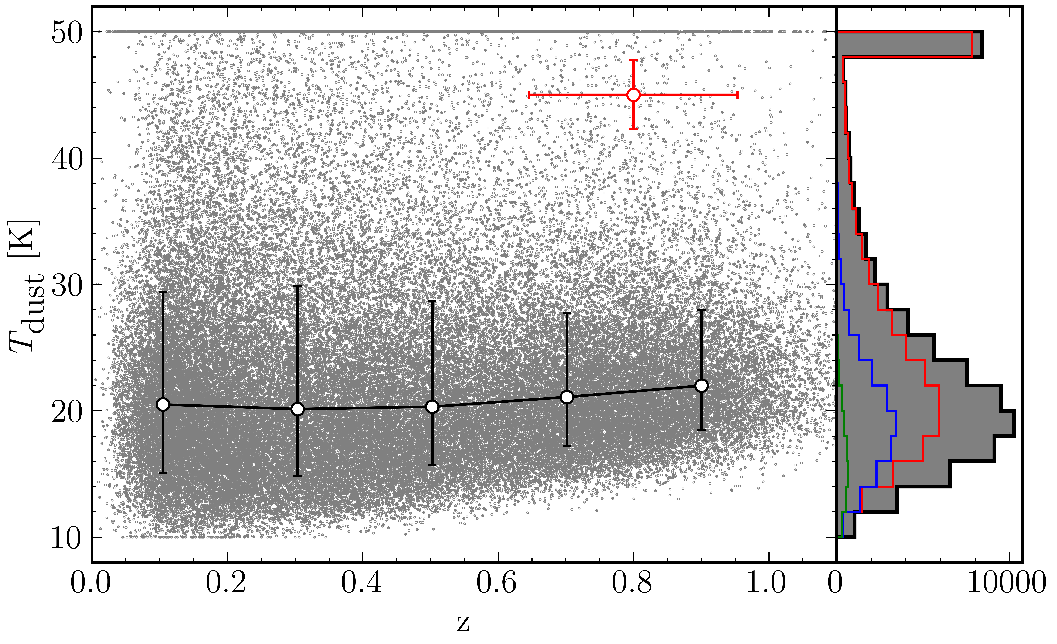
\includegraphics[width=0.9\columnwidth]{Figures/dust_temperatures.pdf}
	\caption{Caption. {\color{red} Complete.}}
	\label{fig:dust_temperatures}
\end{figure}

In subsequent sections we shall use the median temperature of 20\,K when deriving the DMF (e.g. \citealt{Vlahakis_2005}). This is required for certain methods used to derive a binned DMF in $M_{\textrm{dust}}-z$ space as they rely on the knowledge of the modified blackbody SED to apply appropriate k-corrections in each bin (see Section {\color{red} X}). This allows us to use all the galaxies in our sample, regardless of the SNR in the SPIRE wavebands. As will be explained later, some methodologies for binned functions allow for each galaxy to use its own SED rather than a global SED to compute the required k-corrections - we shall discuss how this impacts our DMF by considering the galaxies in the SGP for which the modified blackbodies are well constrained and using those to place constraints on the temperature of the remaining sources. {\color{red} Make sure to do this - e.g. reduce the sample beforehand and recompute PC00 and PC00+D11.}

A dust mass can be calculated from the monochromatic rest frame luminosity, which in turn can be obtained from the observed flux density at a given wavelength. We translate the 250\,\micron flux densities of the SGP galaxies into monochromatic luminosities using

\begin{equation}
    L_{250} = \frac{4\pi D_L^2 S_{250}K}{(1+z)},
\label{eq:monohromatic_luminosities}
\end{equation}

\noindent where $L_{250}$ is in units of W Hz$^{-1}$, $D_L$ is the luminosity distance, $S_{250}$ is the observed flux density and $K$ is the k-correction that allows us to define a rest frame quantity at 250\,\micron in terms of the observed frame at the same wavelength, given by

\begin{equation}
    K = \frac{S_{250}^{K}}{S_{250}^{\textrm{obs}}} = \Bigg(\frac{\nu_{K}}{\nu_{\textrm{obs}}}\Bigg)^{3+\beta}\frac{e^{(h\nu_{\textrm{obs}}/kT)} - 1}{e^{(h\nu_{K}/kT)} - 1},
\label{eq:k_correction}
\end{equation}

\noindent where $\nu_{K} = \nu_{\textrm{obs}}(1+z)$ and $T$ and $\beta$ are the dust temperature and emissivity index describing the SED. Consider a galaxy at the edge of our redshift range, z $\sim$ 1. The factor $K$ allows us to convert $S_{250}^{\textrm{obs}}$, the emission radiated at 250\,\micron (1.2\,THz) and observed at 125\,\micron (2.4\,THz) to $S_{250}^{K}$, the 250\,\micron flux density in the galaxy's rest frame. The monochromatic luminosity at 250\,\micron is converted to a dust mass using

\begin{equation}
    M_{\textrm{dust}} = \frac{L_{250}}{4\pi\kappa_{250}B(\nu_{250}, T)},
\label{fig:dust_mass}
\end{equation}

\noindent where $\kappa_{250}$ is the dust mass absorption coefficient at 250\,\micron. The dust mass absoprtion coefficient is an amalgamation of terms including the efficiency with which the dust grains emit in reference to a perfect blackbody, the size of the dust grains and their mass volume density. As will be discussed in Chapter \ref{chapter:Dust_Evolution} $\kappa_\nu$, the frequency dependence of the absorption coefficient, can be parameterized as a power law with an exponent of $\beta$ and thus the value of $\beta$ naturally encodes these properties. For this reason the value of $\kappa_\nu$ is highly uncertain with a wide range of values being presented in the literature spanning multiple orders of magnitude (\citealt{Clark_2019}). A commonly used value is 0.077\,m$^{2}$kg$^{-1}$ at 850\,\micron (\citealt{Dunne_2000}; \citealt{daCunha_2008}; \citealt{Dunne_2011}) which represents a theoretical value that lies between the expectation for graphite and silicate dust grains (\citealt{Draine_1984}). Assuming $\beta$ = 2 we scale this value to 250\,\micron such that $\kappa_{250}$ = 0.89\,m$^{2}$kg$^{-1}$.

As mentioned earlier, estimating dust masses from sub-mm photometry is advantageous as the Rayleigh-Jeans part of the Planck function is least sensitive to dust temperature and most sensitive to dust mass. In the Rayleigh-Jeans regime ($\lambda_{\textrm{rest}} \gg \frac{hc}{kT}$) the Planck function reduces to $B(\nu_{250}, T) = \frac{2\nu_{250}^{2}kT}{c^2}$ which means that in the optically thin and R-J regimes our dust mass estimates are only linearly dependent on the dust temperature. {\color{red} Comparison of 250 and 350um - use "wavelength selection" section in notes.}

\section{Sources of Incompleteness}

When deriving our DMF we must consider the completeness of our FIR selected survey and account for missing galaxies in our volume density calculations. The DMFs determined from galaxies selected in H-ATLAS will naturally have an incompleteness from the flux-limited sub-mm and optical/near-IR catalogues and from the ID crossmatching (Chapter \ref{chapter:Data_Release_3}). In the following sections we outline the methods used to estimate the completeness correction factors for each sub-mm/near-IR pair in our SGP catalogue. Each object identified in our reliable sample will be multiplied by a correction factor that compensates for missing sub-mm sources and detected sources without counterparts found by our Bayesian LR method. 

\subsection{Sub-mm Catalogue Incompleteness}

The first correction factor results from the source extraction process used to create the sub-mm catalogues from the \textit{Herschel} maps. To determine the completeness of the H-ATLAS catalogues from noisy sub-mm images, \citealt{Valiante_2016} used a catalogue of simulated sources embedded in real H-ATLAS maps to predict the efficacy of the \texttt{MADX} algorithm in recovering the sources. The completeness is shown as a function of the measured 250\,\micron flux density of a given source in Figure \ref{fig:submm_completeness} and is listed in Table \ref{tab:submm_completeness_table} along with the correction factors, $c_{\textrm{sub-mm}}$, defined as the reciprocal of the completeness. We use an interpolated version of this table when applying the correction factors to our SGP galaxies. Unsurprisingly, the correction factors are highest near and below the flux limit of the catalogue where confusion noise dominates and the likelihood of lost sources rises. 

\begin{table}
    \centering
    \begin{tabular}{|p{4.5cm}|p{2.5cm}|p{2.5cm}|}
        \hline
        250\,\micron Flux Density [mJy] & Completeness & $c_{\textrm{sub-mm}}$ \\
        \hline
        \hline
        20.0 & 0.541 & 1.849 \\
        26.5 & 0.762 & 1.313 \\
        35.1 & 0.903 & 1.107 \\
        46.4 & 0.969 & 1.032 \\
        61.5 & 0.989 & 1.011 \\
        81.4 & 0.993 & 1.007 \\
        107.7 & 0.997 & 1.003 \\
        142.6 & 0.997 & 1.003 \\
        188.8 & 0.997 & 1.003 \\
        250.0 & 0.999 & 1.001 \\
        \hline
    \end{tabular}
    \caption{Caption. {\color{red} Complete.}}
    \label{tab:submm_completeness_table}
    \begin{tabular}{|p{4.5cm}|p{2.5cm}|p{2.5cm}|}
        \hline
        Redshift & Completeness & $c_{\textrm{id}}$ \\
        \hline
        \hline
        0.05 & 0.984 & 1.016 \\
        0.15 & 0.881 & 1.135 \\
        0.25 & 0.713 & 1.403 \\
        0.35 & 0.542 & 1.844 \\
        0.45 & 0.432 & 2.313 \\
        0.55 & 0.387 & 2.581 \\
        0.65 & 0.372 & 2.685 \\
        0.75 & 0.360 & 2.776 \\
        0.85 & 0.392 & 2.552 \\
        0.95 & 0.422 & 2.369 \\
        \hline
    \end{tabular}
    \caption{Caption. {\color{red} Complete.}}
    \label{tab:id_completeness_table}
\end{table}

\subsection{Near-IR Catalogue Incompleteness}

A second correction typically applied to FIR derived DMFs results from the incompleteness in the optical/near-IR catalogue as we approach the limiting magnitude of the survey. In the GAMA study of \citealt{Dunne_2011} it is shown that the SDSS catalogue is incomplete as we approach the optical flux limit by extrapolating the slope of the number counts in complete bins to fainter magnitudes. The completeness is then estimated from the difference between the extrapolated number counts at the faintest magnitudes and the observed counts. This method assumed that the SDSS catalogue is close to 100\% completeness between $r$-band magnitudes of 19 -- 21.5. 

This correction is of particular importance for optically selected samples where the fraction of sub-mm sources that do not have associations on the optical images, $1 - Q$, is a significant fraction of the total sample. As shown in Table \ref{tab:data_release_input_surveys}, this fraction is approximately 40 -- 50\% for SDSS, while for the VIKING analysis of the SGP it is only $\sim$ 20\%. In addition, the missing 20\% of near-IR counterparts are likely to be at high redshift with many expected to be beyond the upper limit used in this study (z = 1). {\color{red} Some plot or calculation to illustrate that our missing near-IR objects are at high redshifts. Perhaps Eales+2018 calculation?}

\subsection{Reliable ID Incompleteness}

The final correction function arises from our inability to identify all the near-IR counterparts to a high enough reliability for all the sub-mm sources in which we observe at least one counterpart on the near-IR image. As detailed in the previous chapter, our confidence in selecting the appropriate ID for each source is lowered by positional uncertainties, the possibility of coincident background objects and multiple systems that are physically associated with each other but are treated independently with the current method.

The completeness function of our reliable IDs allow us to correct for the number density of sources that have near-IR counterparts above the limiting magnitude of the VIKING survey, but were not retained in the final sample. In order to estimate the completeness of our reliable sample we use a similar methodology to the one used to calculate the probability distribution of true counterparts, $q(m)$, in Section \ref{sec:true_counterparts_distribution}. To ensure that we are accounting for all objects in our ID sample we measure the completeness function as a function of redshift given that we require this for all galaxies in our DMF calculation. As a means of comparison, we can start with a first order approximation using the fraction of all sub-mm sources where we observe near-IR counterparts and the percentage of these sources that are deemed reliable. We observe VIKING objects for 83\% of sub-mm sources while 57\% are considered in our final sample with R > 0.8. From this we know that approximately 69\% of all \textit{Herschel} galaxies in the SGP are contained within our reliable sample, suggesting that our average ID correction factor, $c_{\textrm{id}} \sim$ 1/0.69 $\sim$ 1.46.

In its simplest form, the completeness of our reliable sample is defined as the number of reliable IDs divided by the true redshift distribution of SPIRE counterparts, scaled to the number of sources for which we observe VIKING counterparts. This second term is closely related to the probability distribution of true counterparts as a function of redshift, $q(z)$. Using the same formalism as in Equation \ref{eq:true_counterparts_distribution}, we define the denominator of our completeness as

\begin{equation}
    n_{\textrm{real, scaled}} = q(z)\times N_{\textrm{250\,\micron}} = \frac{n_{\textrm{real}}(z)}{\sum_{z_i}n_{\textrm{real}}(z_i)}\times QN_{\textrm{250\,\micron}},
\end{equation}

\noindent where $n_{\textrm{real}}(z)$ is the estimated true redshift distribution of the counterparts (see Equation \ref{eq:real_distribution}) and $N_{\textrm{250\,\micron}}$ is the number of SPIRE positions. The ID completeness is then defined as $C_{\textrm{id}} = n_{\textrm{reliable}}(z)/n_{\textrm{real, scaled}}$ where $n_{\textrm{reliable}}(z)$ is the redshift distribution of our IDs, and as previously, the required correction functions are the reciprocal of the completeness. While deriving the $q(m)$ distribution in Section \ref{sec:true_counterparts_distribution} we noted that the distribution is normalized in the above manner such that the integal of $q(m)$ over all magnitudes up to the limiting magnitude of the VIKING survey is equal to the probability that the source is detected ($\int^{m_\textrm{lim}} q(m) dm = Q$). As an extension of this validity check, we recognize that the integral of the ID redshift distribution multiplied by the correction factors should give the total number of sources with observable counterparts (i.e. $\int_z c_{\textrm{id}} n_{\textrm{reliable}}(z) dz = QN_{\textrm{250\,\micron}}$, where $c_{\textrm{id}}$ are the correction factors defined as $1/C_{\textrm{id}}$).

The ID completeness as a function of redshift is listed in Table \ref{tab:id_completeness_table} and illustrated in Figure \ref{fig:id_completeness} alongside the completeness functions from the SDP (\citealt{Smith_2011}), GAMA9 field (\citealt{Fleuren_2012}) and NGP (\citealt{Bourne_2016}). The average correction factor per source in the SGP is approximately two, which is significantly larger than our first order approximation. {\color{red} Does this tell us something interesting?}  Near the median redshift of the VIKING redshift distribution ($z \sim$ 0.5) the completeness is lower in the SGP than in previous studies, though we note that we do not include spectroscopic redshifts and the fraction of IDs with redshifts is different among the studies. {\color{red} Why might this be?} The general trend for all H-ATLAS fields is a steady decline from close to 100\% completeness at $z = 0$ to a minimum at $z \sim$ 0.5 -- 0.7 followed by a rise at higher redshifts. \citealt{Bourne_2016} provide the following explanations for the high completeness at low and high redshifts. First, at low redshifts, a fixed search radius will correspond to a smaller physical scale and thus likely to contain fewer counterparts which would explain some of the steady decline to $z \sim$ 0.5. At higher redshifts the ID completeness rises again suggesting that the probability of identifying a VIKING counterpart is higher at higher redshifts, though this could relate to the larger photometric redshift errors. A possible argument is that at higher redshifts where we approach the magnitude limit of the VIKING survey we are less prone to correlated neighbours which would otherwise reduce the reliability of our ID.

\begin{figure}
	\centering
	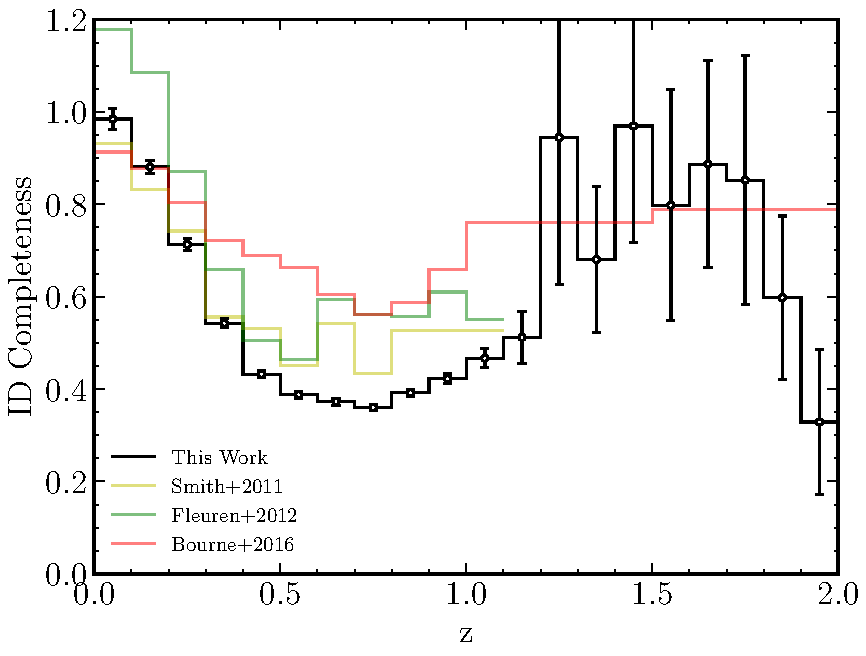
\includegraphics[width=0.75\columnwidth]{Figures/id_completeness.pdf}
	\caption{Caption. {\color{red} Complete and add errors.}}
	\label{fig:id_completeness}
\end{figure}

\section{Estimators of the Binned Dust Mass Function}

The dust mass function, $\phi$, represents the space density of galaxies as a function of dust mass, which in its differential form is defined as the number of galaxies per unit comoving volume per unit dust mass interval:

\begin{equation}
    \phi(M_{\textrm{dust}}, z) = \frac{d^2N}{dV dM_{\textrm{dust}}},
\label{eq:differential_phi}
\end{equation}

\noindent where $N$ is the number of galaxies with dust mass $M_{\textrm{dust}}$ observed in the comoving volume $V$ at redshift $z$. In this section we outline two methods of calculating the binned dust mass function; the ubiquitously used $1/V_{\textrm{max}}$ method (\citealt{Schmidt_1968}; \citealt{Felten_1976}; \citealt{Avni_1980}) and the approximate method, $\phi_{\textrm{est}}$, proposed by \citealt{Page_2000}. Alternative parametric methods (e.g. the maximum-likelihood method of \citealt{Marshall_1983}) allow us to explore the entire $M_{\textrm{dust}} - z$ space, including regions not covered by observational data, and produce continuous functions for $\phi(M_{\textrm{dust}}, z)$. Although it is well established that the dust mass function can be parameterized in the form of a Schechter function, it is not obvious how this function evolves with redshift and which functional form should be used for this evolution. For this reason, we prefer to use a binned non-parametric method and empirically study the redshift evolution of the DMF.

\subsection{The $1/V_{\textrm{max}}$ Method}

The prevalent use of the $1/V_{\textrm{max}}$ method stems from our need to overcome the Malmquist bias (\citealt{Eddington_1914}; \citealt{Malmquist_1922}) that causes selection biases in flux density limited samples. At a given redshift the faintest galaxies are statistically more likely to be left out of the survey, while the most luminous galaxies can be observed at a greater distance. As a result, there is an observational mass bias in which faint and thus low-mass galaxies are only detected in smaller volumes compared to brighter galaxies. The $1/V_{\textrm{max}}$ method corrects for this bias by weighting each galaxy according to the maximum comoving volume in which it can be observed by the survey. The number density of galaxies in a given dust mass-redshift bin ($\Delta M_{\textrm{dust}} \Delta z$) is approximately given by the summation of the reciprocal of the maximum comoving volume for all galaxies in this bin:

\begin{equation}
    \frac{dN}{dV} \sim \sum_{i=1}^N \frac{1}{V_{\textrm{max,i}}(M_{\textrm{dust,i}},z)},
\label{eq:number_density_1/v_method}
\end{equation}

\noindent where $V_{\textrm{max,i}}$ is the maximum comoving volume (up to the maximum redshift of the bin) in which the $i$th galaxy in this bin could be detected in the survey. The volume is calculated according to

\begin{align}
    V_{\textrm{max},i}(M_{\textrm{dust,i}},z) &= \int^{\scriptscriptstyle \textrm{survey}} \int_{\scriptscriptstyle z_1}^{\scriptscriptstyle \textrm{min}[z_2, z(M_{\textrm{dust,i}},S_{\textrm{lim}})]} \frac{dV}{dz} dz d\Omega \nonumber \\
    &= \int^{\scriptscriptstyle \textrm{survey}} \int_{\scriptscriptstyle z_1}^{\scriptscriptstyle \textrm{min}[z_2, z(M_{\textrm{dust,i}},S_{\textrm{lim}})]} D_H \frac{(1+z)^2 D_A^2}{E(z)} dz d\Omega
\label{eq:volume_1/v_method}
\end{align}

\noindent where $\frac{dV}{dz}$ is the differential comoving volume given in the following line in terms of the Hubble distance, $D_H$, the angular diameter distance, $D_A$, and the dimensionless Hubble parameter, $E(z)$. The integration over redshift has a lower limit of the bottom redshift of the bin, $z_1$, and an upper limit of either the upper edge of the bin, $z_2$, or the redshift beyond which the galaxy with dust mass $M_{\textrm{dust},i}$ would not be observed, whichever is smallest. A graphical illustration of the integration used to calculate the volume is presented in the left-hand panel of Figure \ref{fig:volume_comparison}.

The dust mass function using this method is then defined by dividing the number density by the dust mass bin width (which we define in terms of logarithmic dust mass):

\begin{equation}
    \phi_{1/V}(M_{\textrm{dust}},z) = \frac{1}{\Delta \textrm{log}_{10}(M_{\textrm{dust}})} \sum_{i=1}^N \frac{1}{V_{\textrm{max,i}}(M_{\textrm{dust,i}},z)}.
\label{eq:phi_1/v_method}
\end{equation}

To account for the incompleteness of the sample we can include our correction factors from the previous sections in the following way:

\begin{equation}
    \phi_{1/V}(M_{\textrm{dust}},z) = \frac{1}{\Delta \textrm{log}_{10}(M_{\textrm{dust}})} \sum_{i=1}^N \frac{c_{\scriptscriptstyle \textrm{sub-mm}} c_{\scriptscriptstyle \textrm{id}}}{V_{\textrm{max,i}}(M_{\textrm{dust,i}},z)}.
\label{eq:phi_1/v_method}
\end{equation}

While this method suitably deals with Malmquist bias and is a non-parametric technique that does not require an analytic form, it can produce some unwanted artefacts when applied to flux-limited samples. An alternative method that better handles objects close to the flux limit of the survey is the method of \citealt{Page_2000} (hereafter PC00).

\subsection{The Page and Carrera Method}

In the $1/V_{\textrm{max}}$ method we assume that the accessible comoving volume in which a galaxy could have been detected by the survey is constant across all dust masses in a given $M_{\textrm{dust}} - z$ bin. The following method has the advantage that the comoving volume is defined from the average value for all dust masses in the interval $\Delta M_{\textrm{dust}}$. In a similar fashion as before, the number density of galaxies is approximately given by the sum of all galaxies in the bin divided by the average accessible volume, 

\begin{equation}
    \frac{dN}{dV} \sim \frac{\sum_{i=1}^N 1}{V_{\textrm{max,av}}(M_{\textrm{dust}},z)},
\label{eq:number_density_pc00_method}
\end{equation}

\noindent where $V_{\textrm{max,av}}$ now represents an average volume for all galaxies in the interval $\Delta M_{\textrm{dust}} \Delta z$. This volume is averaged over all dust masses in the bin following

\begin{multline}
    V_{\textrm{max,av}}(M_{\textrm{dust}},z) = \frac{1}{\Delta \textrm{log}_{10}(M_\textrm{dust})}\int_{\scriptscriptstyle M_{\textrm{dust,1}}}^{\scriptscriptstyle M_{\textrm{dust,2}}} \int^{\scriptscriptstyle \textrm{survey}} \int_{\scriptscriptstyle z_1}^{\scriptscriptstyle \textrm{min}[z_2, z(M_{\textrm{dust}},S_{\textrm{lim}})]} \\ D_H \frac{(1+z)^2 D_A^2}{E(z)} dz d\Omega d\textrm{log}_{10}(M_\textrm{dust}),
\label{eq:volume_pc00_method}
\end{multline}

\noindent which is akin to Equation \ref{eq:volume_1/v_method}, except we integrate over all dust masses and divide by the bin width. Crucially this means that we are not dependent on any individual estimate of the dust mass, $M_{\textrm{dust,i}}$. A comparison with the volume calculation in the $1/V_{\textrm{max}}$ method is shown in the right-hand panel of Figure \ref{fig:volume_comparison}. In the same process as before, the dust mass function is defined as the number density divided by the dust mass bin width:

\begin{align}
    \phi_{\textrm{est}}(M_{\textrm{dust}},z) &= \frac{1}{\Delta \textrm{log}_{10}(M_{\textrm{dust}})} \times \nonumber \\
    & \qquad \frac{\sum_{i=1}^N c_{\scriptscriptstyle \textrm{sub-mm}} c_{\scriptscriptstyle \textrm{id}}}{\frac{1}{\Delta \textrm{log}_{10}(M_\textrm{dust})}\int_{\scriptscriptstyle M_{\textrm{dust,1}}}^{\scriptscriptstyle M_{\textrm{dust,2}}} \int^{\scriptscriptstyle \textrm{survey}} \int_{\scriptscriptstyle z_1}^{\scriptscriptstyle \textrm{min}[z_2, z(M_{\textrm{dust}},S_{\textrm{lim}})]} D_H \frac{(1+z)^2 D_A^2}{E(z)} dz d\Omega d\textrm{log}_{10}(M_\textrm{dust})} \nonumber \\
    &= \frac{\sum_{i=1}^N c_{\scriptscriptstyle \textrm{sub-mm}} c_{\scriptscriptstyle \textrm{id}}}{\int_{\scriptscriptstyle M_{\textrm{dust,1}}}^{\scriptscriptstyle M_{\textrm{dust,2}}} \int^{\scriptscriptstyle \textrm{survey}} \int_{\scriptscriptstyle z_1}^{\scriptscriptstyle \textrm{min}[z_2, z(M_{\textrm{dust}},S_{\textrm{lim}})]} D_H \frac{(1+z)^2 D_A^2}{E(z)} dz d\Omega d\textrm{log}_{10}(M_\textrm{dust})}
\label{eq:phi_pc00_method}
\end{align}

In the above formalism (hereafter PC00), the accessible volume is calculated for each $M_{\textrm{dust}} - z$ bin assuming a global SED to translate the flux limit of the survey to a limiting dust mass at each redshift. This means that all galaxies in a bin are assumed to follow the same $M_{\textrm{dust}} - z$ relationship. \citealt{Dunne_2011} present a modified version of the PC00 method that allows each galaxy to set its own limiting $M_{\textrm{dust}} - z$ relationship, allowing for the range of SEDs in each bin. In this form, each galaxy has an individual contribution to the dust mass function that are then summed within the bin such that

\begin{equation}
    \phi_{\textrm{est, Dunne}}(M_{\textrm{dust}},z) = \sum_{i=1}^N \frac{c_{\scriptscriptstyle \textrm{sub-mm}} c_{\scriptscriptstyle \textrm{id}}}{\int_{\scriptscriptstyle M_{\textrm{dust,1}}}^{\scriptscriptstyle M_{\textrm{dust,2}}} \int^{\scriptscriptstyle \textrm{survey}} \int_{\scriptscriptstyle z_1}^{\scriptscriptstyle \textrm{min}[z_2, z(M_{\textrm{dust}},S_{\textrm{lim,i}})]} D_H \frac{(1+z)^2 D_A^2}{E(z)} dz d\Omega d\textrm{log}_{10}(M_\textrm{dust})},
\label{eq:phi_pc00_dunne_method}
\end{equation}

\noindent where the integration over redshift is computed individually for each source. This has the added benefit of allowing a unique flux limit to be used for each galaxy $S_{\textrm{lim,i}}$, which is useful for surveys like H-ATLAS where source extraction is based on the SNR of the source rather than a single flux cut.

\subsection{Comparison of Estimators}

While the $1/V_{\textrm{max}}$ estimator is a suitable way of accounting for Malmquist bias, the PC00 method provides additional advantages for far-IR derived DMFs. Firstly, the accessible volume is not dependent on the dust mass of any individual galaxy, which can have significant uncertainties due to flux boosting. Second, the approach to calculating the accessible volume using the two estimators causes differences in underpopulated bins near the flux limit of the survey. Figure \ref{fig:volume_comparison} shows a comparison of the accessible volume calculations for an example $M_{\textrm{dust}} - z$ bin ($8 < \textrm{log}_{10}(M_\textrm{dust}) < 8.25, 0.2 < z < 0.4$). In this exemplar undersampled bin, the volume calculated from the $1/V_{\textrm{max}}$ will typically be an overestimate of the true region of the dust mass-volume space that has been surveyed, leading to an underestimate of the DMF in the least massive bin of any given redshift slice. In bins that correspond to all objects being brighter than the flux limit of the survey, the volume estimates yield the same result and we expect the DMFs to be identical.

\begin{figure}
	\centering
	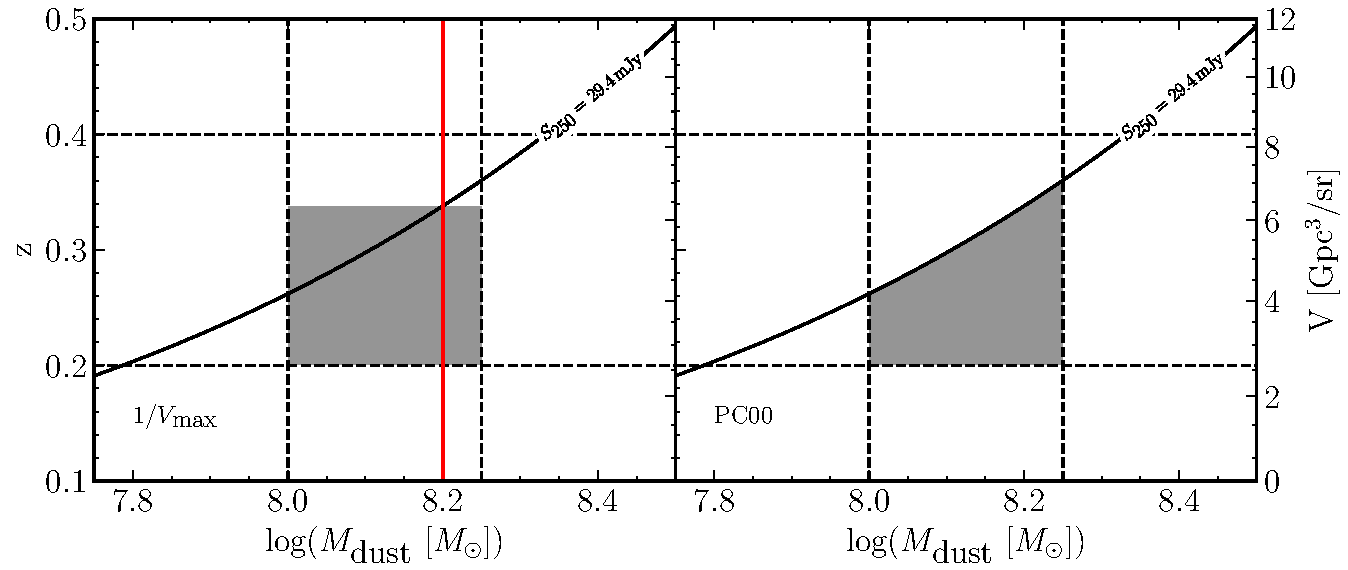
\includegraphics[width=\columnwidth]{Figures/volume_comparison.pdf}
	\caption{Caption}
	\label{fig:volume_comparison}
\end{figure}

\section{The Dust Mass Function from Galaxies in the SGP}

We apply the methods described above to the galaxies observed in the SGP field of H-ATLAS. It is important to note that our sample is devoid of spectroscopic redshifts and our dust masses are derived from sub-mm fluxes that are susceptible to flux boosting. The scatter in dust masses due to their measurement uncertainty could move galaxies between neighbouring bins in either direction. Given that the volume density is not uniform across bins and the survey is flux-limited, this can introduce an Eddington bias (\citealt{Eddington_1913}) that broadens the DMF. For this reason, we model the errors as being formed in two parts. First, a Poissonian error that scales as $\sigma_{\phi,N} = \frac{1}{\sqrt{N}}$, where $N$ is the number of galaxies in each bin. The second error term is due to the spread in dust masses as a result of the large uncertainties on our photometric redshifts. When measuring the DMF we run {\color{red} X} Monte Carlo simulations in which we remeasure the DMF having perturbed the redshift of each galaxy according to a Gaussian distribution with standard deviation equal to the error value. We use the standard deviation in the range of $\phi$ we observe in each $M_{\textrm{dust}} - z$ bin and add this error in quadrature to the Poissonian error: $\sigma_\phi = \sqrt{\sigma_{\phi,N}^2 + \sigma_{\phi,z}^2}$.

{\color{red} Go back to here for rewriting}

Figure \ref{fig:dmf_methods} shows the DMF derived using the PC00 (solid lines, filled circles) and $1/V_{\textrm{max}}$ (dotted lines, filled circles) estimators in bins of width 0.2 in redshift from zero to one, assuming a universal dust temperature of 20\,K and dust emissivity index, $\beta$ = 2. As a single SED is being used to measure the dust properties, we must assume a single survey flux limit for all galaxies - which we take to be 29.4\,mJy at 250\,\micron\ (\citealt{Valiante_2016}). As one would expect from bins in which the interval $\Delta M_{\textrm{dust}} \Delta z$ corresponds to objects brighter than the flux limit of the survey, the two estimators are equivalent. However, for $\phi_{1/V}$ there is a downturn in the lowest dust mass bin in most redshift slices, as predicted earlier. The low-mass end of the DMF is typically paramterized as a powerlaw with a slope, $\alpha$, with values between -2 and -1. Our DMF implies a much flatter value, suggesting that the number density of objects between dust masses of $10^{5.5}$ and $10^{7.5}\,M_{\odot}$ is near constant. In light of previous H-ATLAS studies, we expect that this is not physical but rather an indication of an incomplete sample at the lowest masses. Given we are not using spectroscopic redshifts in our sample we are likely missing these systems and therefore in subsequent analysis we shall assume that our DMFs are accurate above $\sim 10^{7.5}\,M_{\odot}$ and use the results of \citealt{Beeston_2018} to fill in this low-mass regime. 

Considering for now the PC00 (T = 20\,K) estimate of the DMF, henceforth $\phi_{\textrm{est, T=20\,K}}$, we 

{\color{red} Describe the general shape - evolution to higher masses etc.}

{\color{red} PC00+D11 method}

The bottom panel of Figure \ref{fig:pc00_vmax_t20} illustrates the fractional error budget, $\sigma_\phi/\phi$, as a function of dust mass for the two uncertainty components: Poisson noise and photometric redshift uncertainty. We have assumed for now the contributions to the PC00 estimator, $\phi_{\textrm{est}}$, as both methods result in similar error distributions. {\color{red} Check that this is true.} The Poissonian fractional error is a reflection of the counts in each bin and thus the highest contributions occur at the high and low mass end of the DMF where the counts are lowest. 

{\color{red} Comment about the shape of the photometric redshift contribution when ready.} 

\begin{figure}
	\centering
	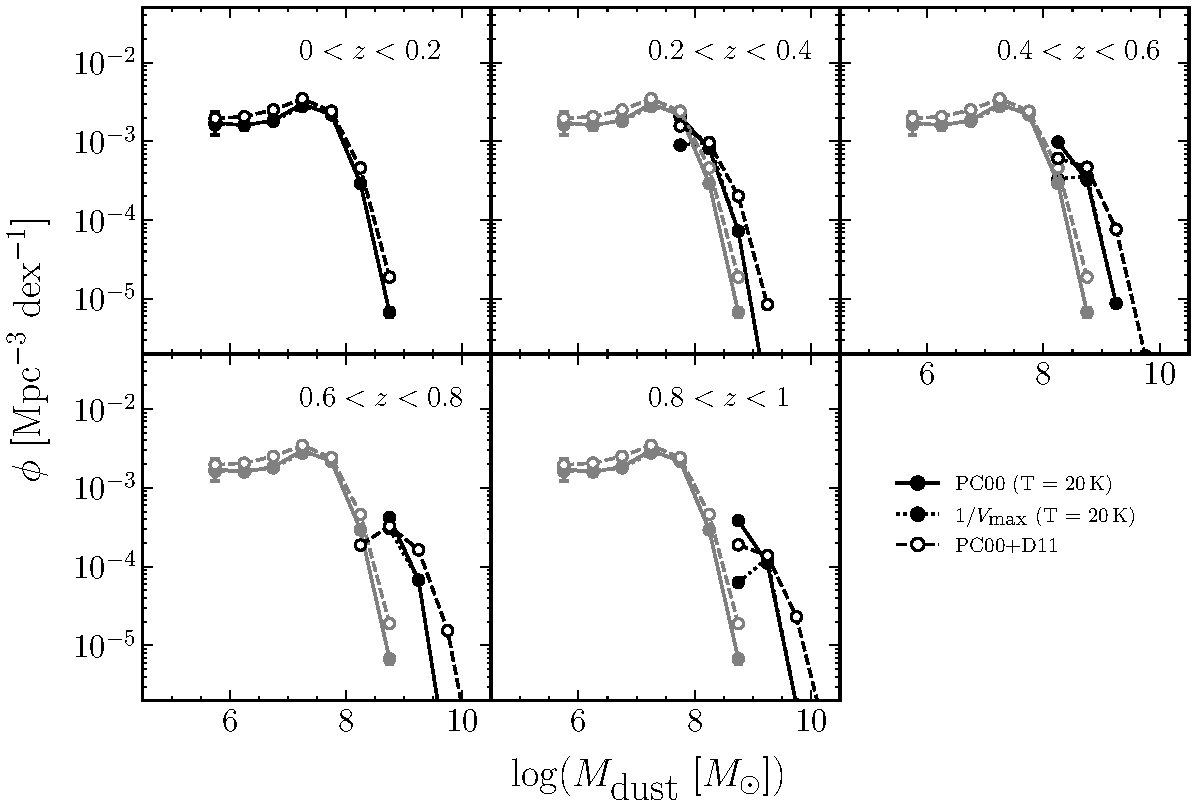
\includegraphics[width=0.9\columnwidth]{Figures/dmf_methods.pdf}
	\caption{Caption.}
	\label{fig:dmf_methods}
\end{figure}

%As an extension to the PC00 method, we would like to be able to use the estimator of \citealt{Dunne_2011} (Equation \ref{eq:phi_pc00_dunne_method}) in which we calculate the acessible volume individually for each source rather than for each bin in the $M_{\textrm{dust}}-z$ plane. The problem we face is that this requires knowing the dust temperatures of all galaxies in our sample. While we are confident about the dust temperatures for a subset of our sample, we cannot depend on these sources alone as we would be introducing an incompleteness to our DMF estimate that is non-trivial to account for. Instead, we shall use these galaxies to define an empirical relationship that will be applied in cases where the full SED could not be fitted. To ensure we select sources for which we have reasonable confidence in their dust temperature, we require that the SED is well-sampled around the peak of the dust emission. 



